% This file was created by matlab2tikz v0.4.4 running on MATLAB 8.1.
% Copyright (c) 2008--2013, Nico Schlömer <nico.schloemer@gmail.com>
% All rights reserved.
% 
% The latest updates can be retrieved from
%   http://www.mathworks.com/matlabcentral/fileexchange/22022-matlab2tikz
% where you can also make suggestions and rate matlab2tikz.
% 
\tikzsetnextfilename{plots/complexBar_eps}
%
% defining custom colors
\definecolor{mycolor1}{rgb}{0.313725501298904,0.313725501298904,0.313725501298904}%
\definecolor{mycolor2}{rgb}{0.941176474094391,0.941176474094391,0.941176474094391}%
%
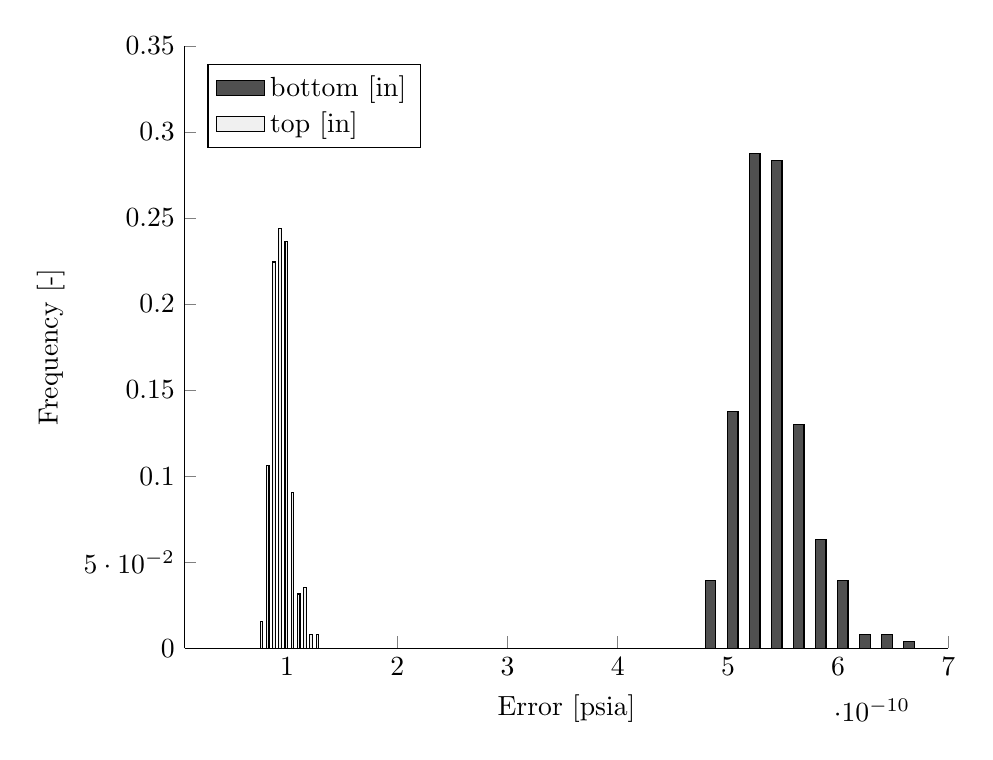
\begin{tikzpicture}

\begin{axis}[%
width=0.8\textwidth,
height=0.630967741935484\textwidth,
area legend,
scale only axis,
xmin=7e-12,
xmax=7e-10,
xlabel={Error [psia]},
ymin=0,
ymax=0.35,
ylabel={Frequency [-]},
axis x line*=bottom,
axis y line*=left,
legend style={at={(0.03,0.97)},anchor=north west,draw=black,fill=white,legend cell align=left}
]
\addplot[ybar,bar width=0.01087013866087131\textwidth,bar shift=-0.00366883666304457\textwidth,draw=black,fill=mycolor1] plot coordinates{(4.87585793962353e-10,0.0393700787401575)
(5.07560571350041e-10,0.137795275590551)
(5.27535348737729e-10,0.28740157480315)
(5.47510126125417e-10,0.283464566929134)
(5.67484903513105e-10,0.12992125984252)
(5.87459680900793e-10,0.062992125984252)
(6.07434458288481e-10,0.0393700787401575)
(6.27409235676168e-10,0.0078740157480315)
(6.47384013063856e-10,0.0078740157480315)
(6.67358790451544e-10,0.00393700787401575)};

\addlegendentry{bottom [in]};

\addplot [
color=black,
solid,
forget plot
]
table[row sep=crcr]{
7e-11 0\\
7e-10 0\\
};
\addplot[ybar,bar width=0.00265379546791768\textwidth,bar shift=0.00103362216744855\textwidth,draw=black,fill=mycolor2] plot coordinates{(7.59143858886091e-11,0.015748031496063)
(8.15418843558291e-11,0.106299212598425)
(8.71693828230491e-11,0.224409448818898)
(9.27968812902691e-11,0.244094488188976)
(9.84243797574891e-11,0.236220472440945)
(1.04051878224709e-10,0.0905511811023622)
(1.09679376691929e-10,0.031496062992126)
(1.15306875159149e-10,0.0354330708661417)
(1.20934373626369e-10,0.0078740157480315)
(1.26561872093589e-10,0.0078740157480315)};

\addlegendentry{top [in]};

\end{axis}
\end{tikzpicture}%
